\section[Jaderně-fyzikální metody v nukleární medicíně]{Jaderně-fyzikální metody v nukleární medicíně: gama kamera, CT, PET}

Jedná se o metody založené na využití farmaceutických radionuklidů, a to ve formě absorpce v těle nebo zavedenímm do lidského organismu. Jako detektory jsou většinou využívány scintilátory, proto metody dělíme na:

\begin{itemize}
    \item dynamickou scintilografii -- sleduje časové změny rozložení radionuklidů, např. činnost orgánů,
    \item planární scintilografie -- statická vizualizace.
\end{itemize}

\subsection{Zdroje záření}

V medicíně lze využívat růzzné druhy zdrojů:

\begin{itemize}
    \item radionuklidy 
    \begin{itemize}
        \item $\gamma$ záření z jaderných reakcí, jsou definovány energií a poločasem rozpadu, musí být vyráběny např. na cyklotronech,
        \item $^{99m}$Tc -- $\gamma$-kamery, $^{18}$F -- PET, $^{123}$I -- $\gamma$-kamera, $^{131}$I -- terapeutický zdroj (prostě ti to vysmaží mutující buňky v nádoru), $^{11}$C -- PET, $^{67}$Ga -- $\gamma$-kamera, $^{81}$Rb -- PET\\
        
        \textit{každý ten zdroj se používá na něco trochu jiného, na diagnostiku mozku použijí asi nějaký jiný než na diagnostiku sleziny atd.}
    \end{itemize}
\end{itemize}

\subsection{Diagnostika}

Dělíme podle činnosti:

\begin{itemize}
    \item morfologická (uspořádání, tvar, velikost),
    \item funkční (činnost orgánů),
    \item dynamická (časová závislost).
\end{itemize}

Podle uspořádání:

\begin{itemize}
    \item absorpční -- RTG, CT,
    \item emisní -- PET, gamma kamera, magnetická rezonance,
    \item kombinovaná -- NAA, CT+PET.
    
\end{itemize}

\subsection{Gamma kamera}

\begin{figure}[H]
    \centering
    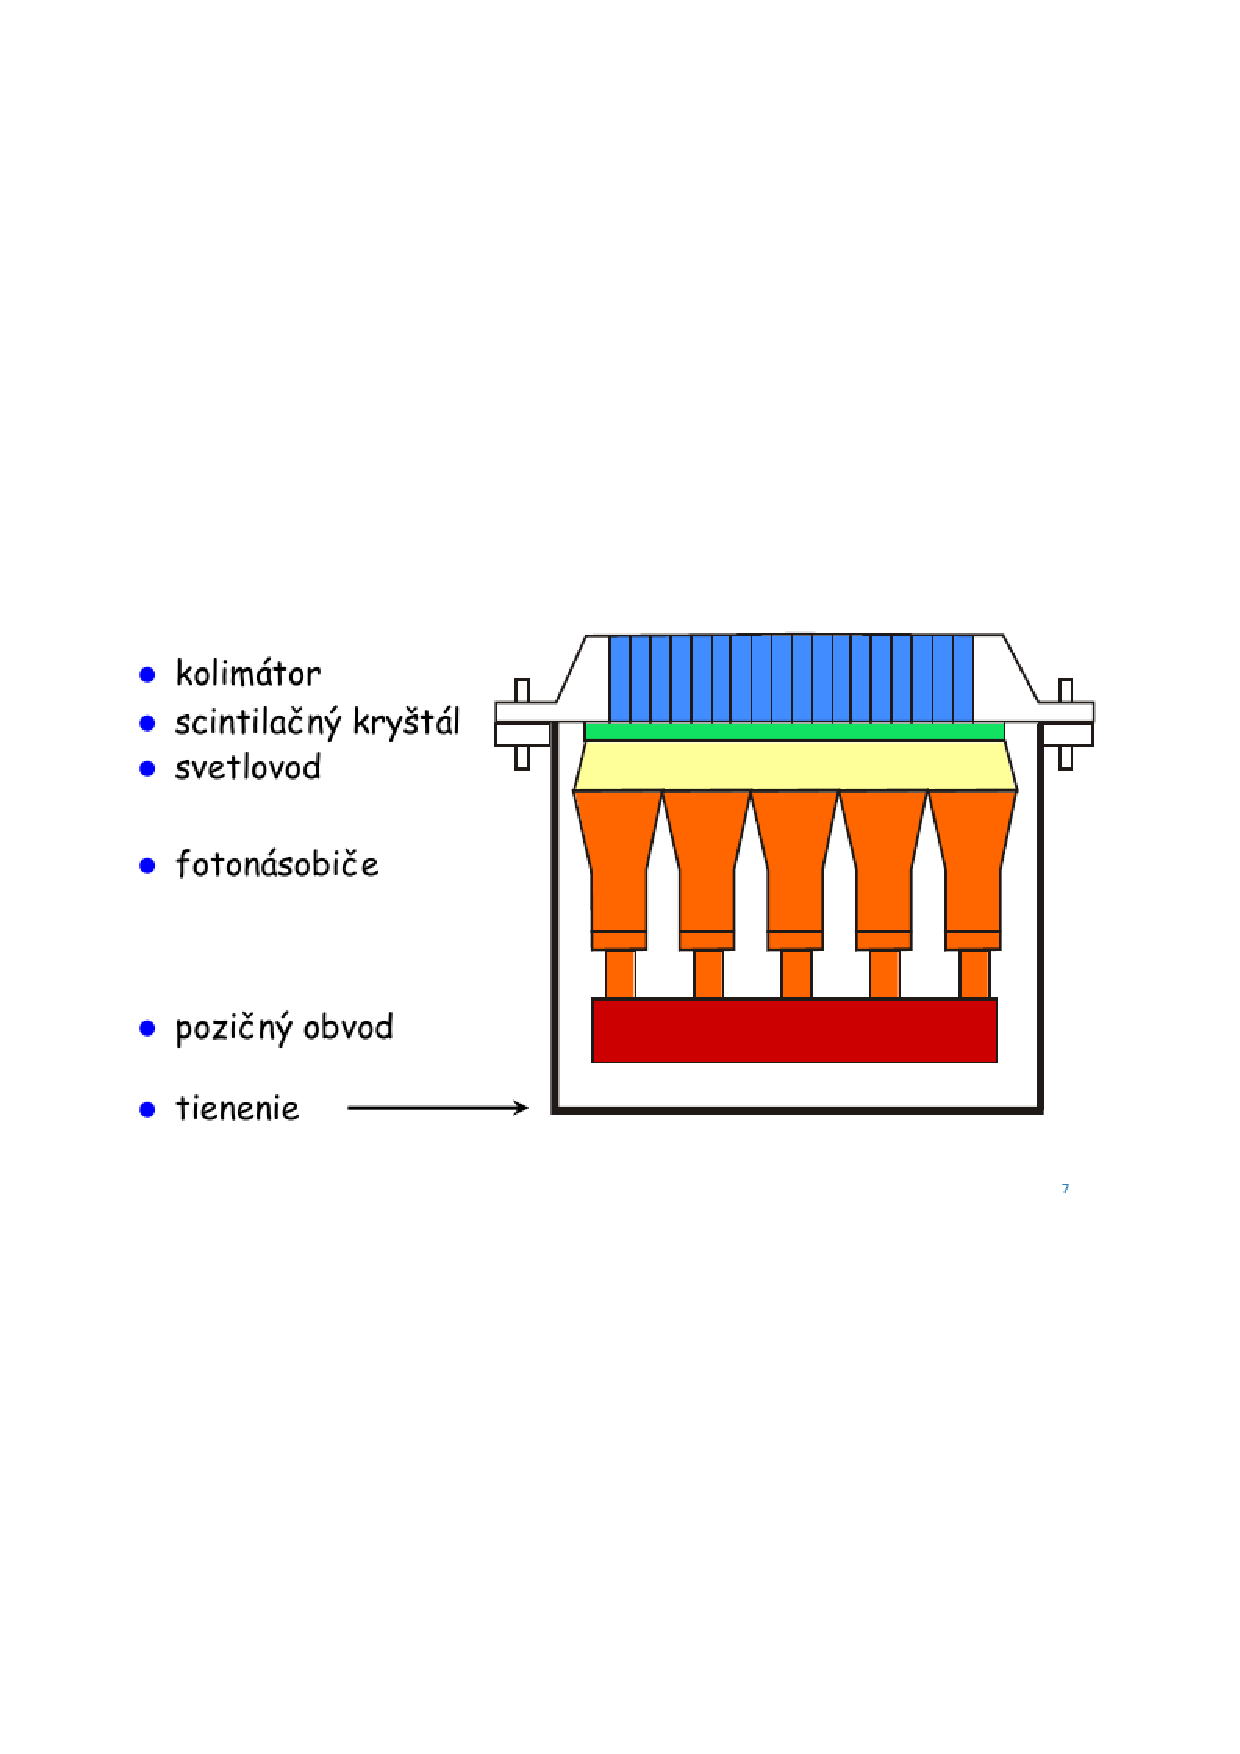
\includegraphics[width=0.55\linewidth, trim={2cm 10cm 2cm 10cm}, clip]{img/gamma_kamera.pdf}
    \caption{Základní komponenty gamma kamery}
    \label{fig:2_5_gamma_kamera}
\end{figure}

\begin{figure}[H]
    \centering
    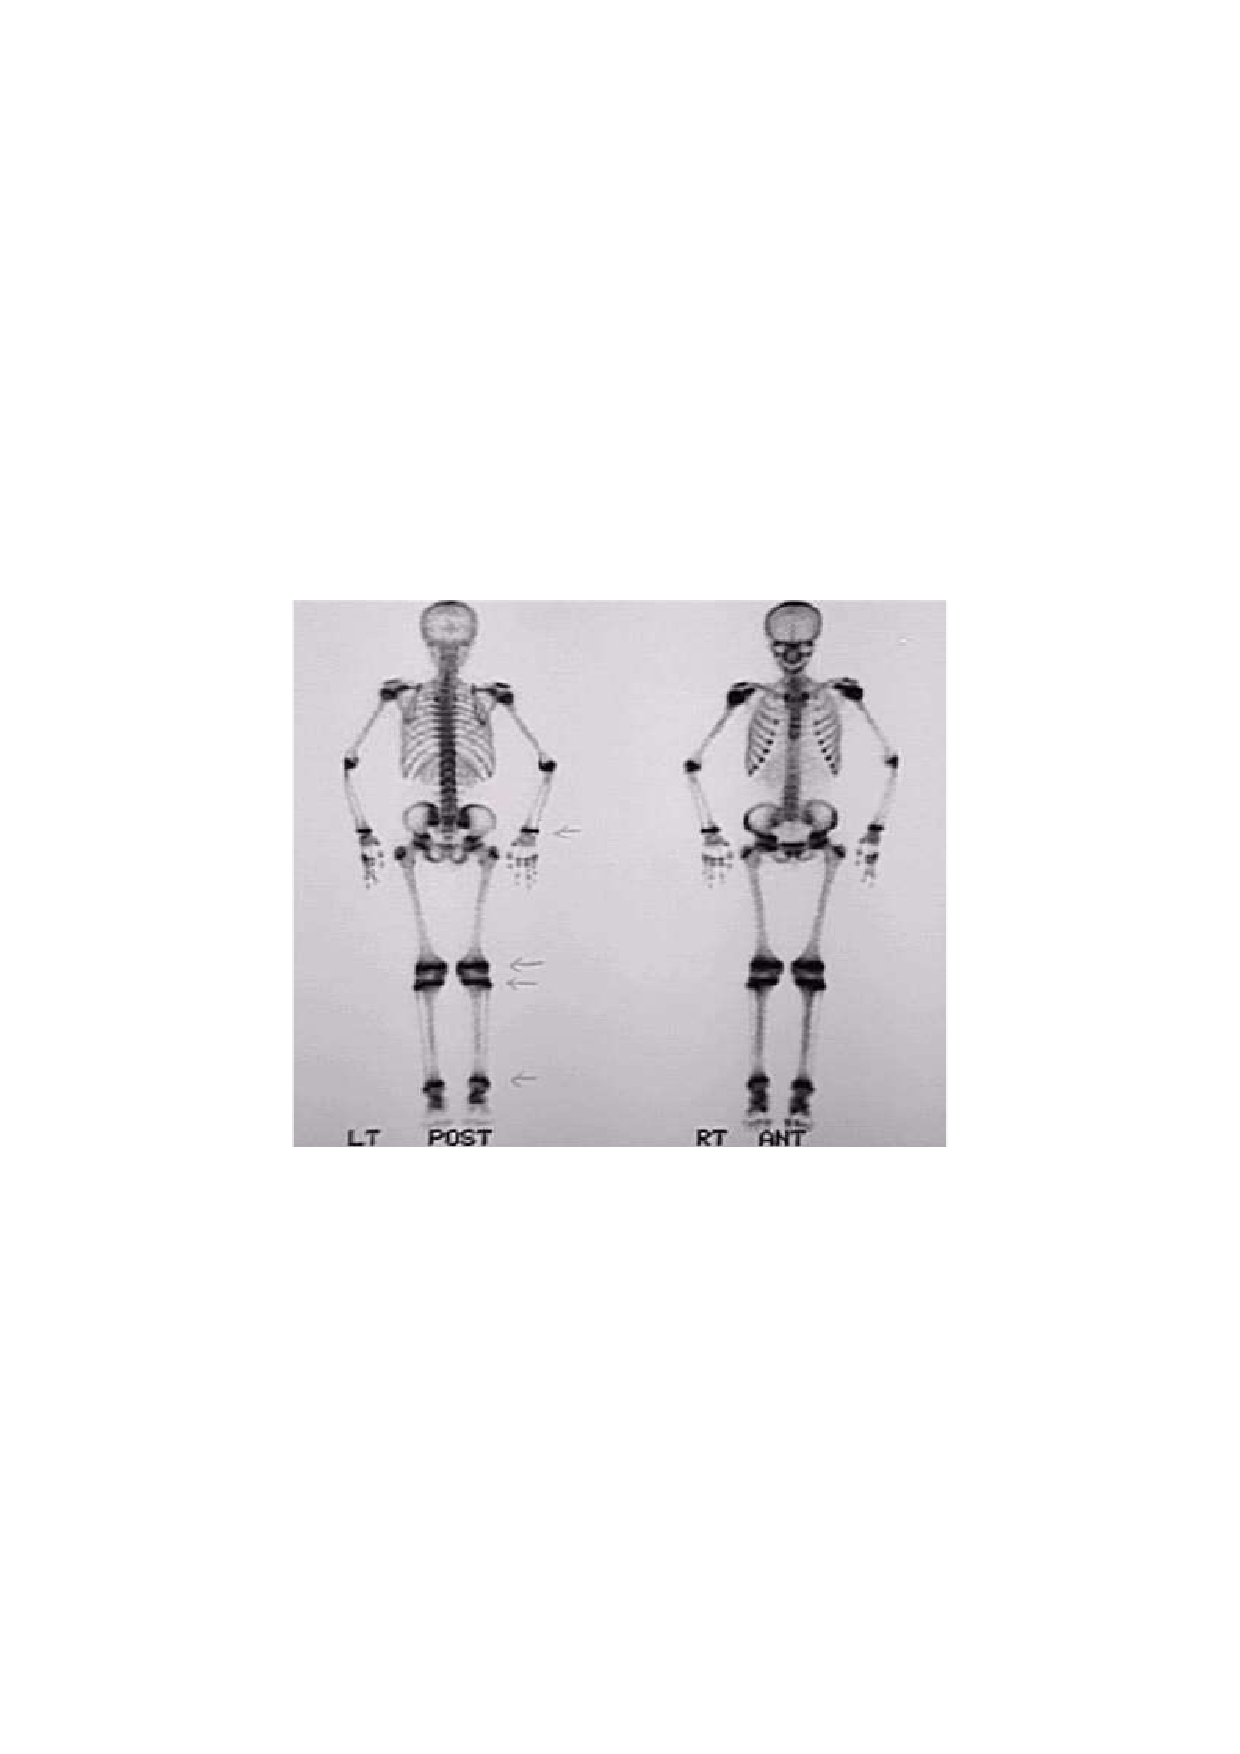
\includegraphics[width=0.5\linewidth, trim={2cm 8cm 2cm 8cm}, clip]{img/gamma_kamera_snimek.pdf}
    \caption{Celotělový snímek z gamma kamery}
    \label{fig:5_2_gamma_kamera_snimek}
\end{figure}

Kolimátor:

\begin{itemize}
    \item paralelní mnohokanálový kolimátor $\rightarrow$ ovlivní směr fotonů, geometické zorné pole kamery, prostorov rozptyl, citlivost systému -- výběr dle energie registrovaných fotonů, rozlišení, skenovací hloubky a požadované citlivosti
    \item výsledný obraz -- počet otvorů, průměr otvorů, délka jednotlivých trubic, materiál atd.
\end{itemize}

Výběr radionuklidu:

\begin{itemize}
    \item poločas rozpadu musí mít několik hodin, produkované $\gamma$ musí ít stovky keV, lehko zabudovatelný do farmaka, v nemocnici musí vydržet několik dní
    \item typicky se používá $^{99m}$Tc
\end{itemize}

\subsection{Počítačová tomografie -- CT}

\subsubsection{Princip}

Zzaložená na zeslabení svazku RTG záření (absorpční metoda):

$$ I = I_0 \cdot exp(-\mu\cdot t). $$

CT: mám sadu $j$ řádků a $i$ sloupců, každý detektor sbírá informaci o zeslabení

$$I_{12} = I_{0} \cdot exp(-(\mu_{1} + \mu_{2})\cdot \Delta t)$$
$$I_{34} = I_{0} \cdot exp(-(\mu_{3} + \mu_{4})\cdot \Delta t)$$
$$I_{13} = I_{0} \cdot exp(-(\mu_{1} + \mu_{3})\cdot \Delta t)$$
$$I_{24} = I_{0} \cdot exp(-(\mu_{2} + \mu_{4})\cdot \Delta t)$$

Přes získané intenzity $I_{12}, I_{34}, I_{13}, I_{24}$ jsem schopný zrekonstruovat koeficienty $\mu_{i}$ ve všech blocích. Ve skutečnosti je ale bloků výrazně více

Generované RTG záření prochází tělem, na druhé straně gantry jsou detekován sadou scintilátorů. Získané data tvoří projekci, kompletní sada zeslabení v závislosti na úhlu $\theta$ a vzdálenosti $t$ je pak sinogram. Následně je obraz rekonstruován.

Sinogram je kompletní soubor projekcí, ukazuje grafickou závislost polohy objektu od úhlu projekce.

\begin{figure}[H]
    \centering
    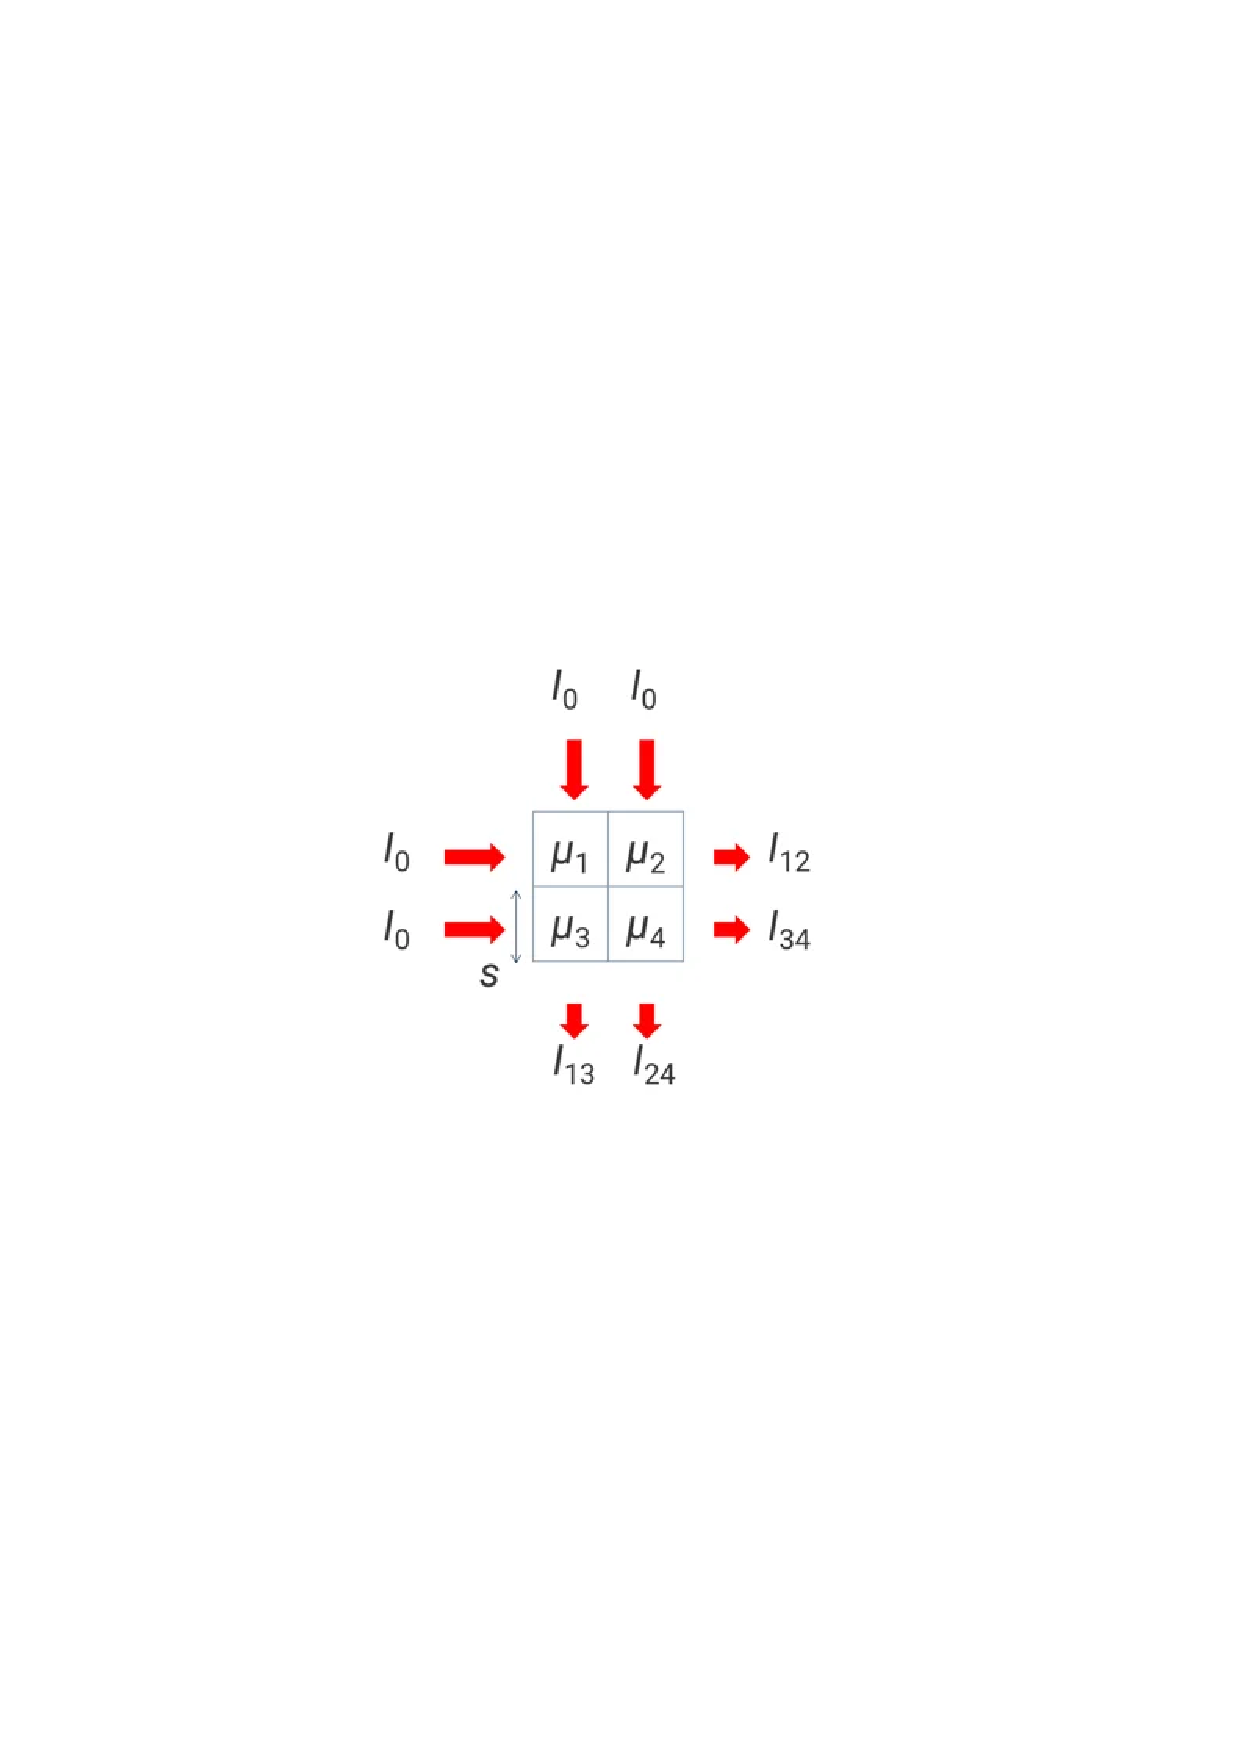
\includegraphics[width=0.4\linewidth,trim={5cm 10cm 5cm 10cm}, clip]{img/ct_scheme.pdf}
    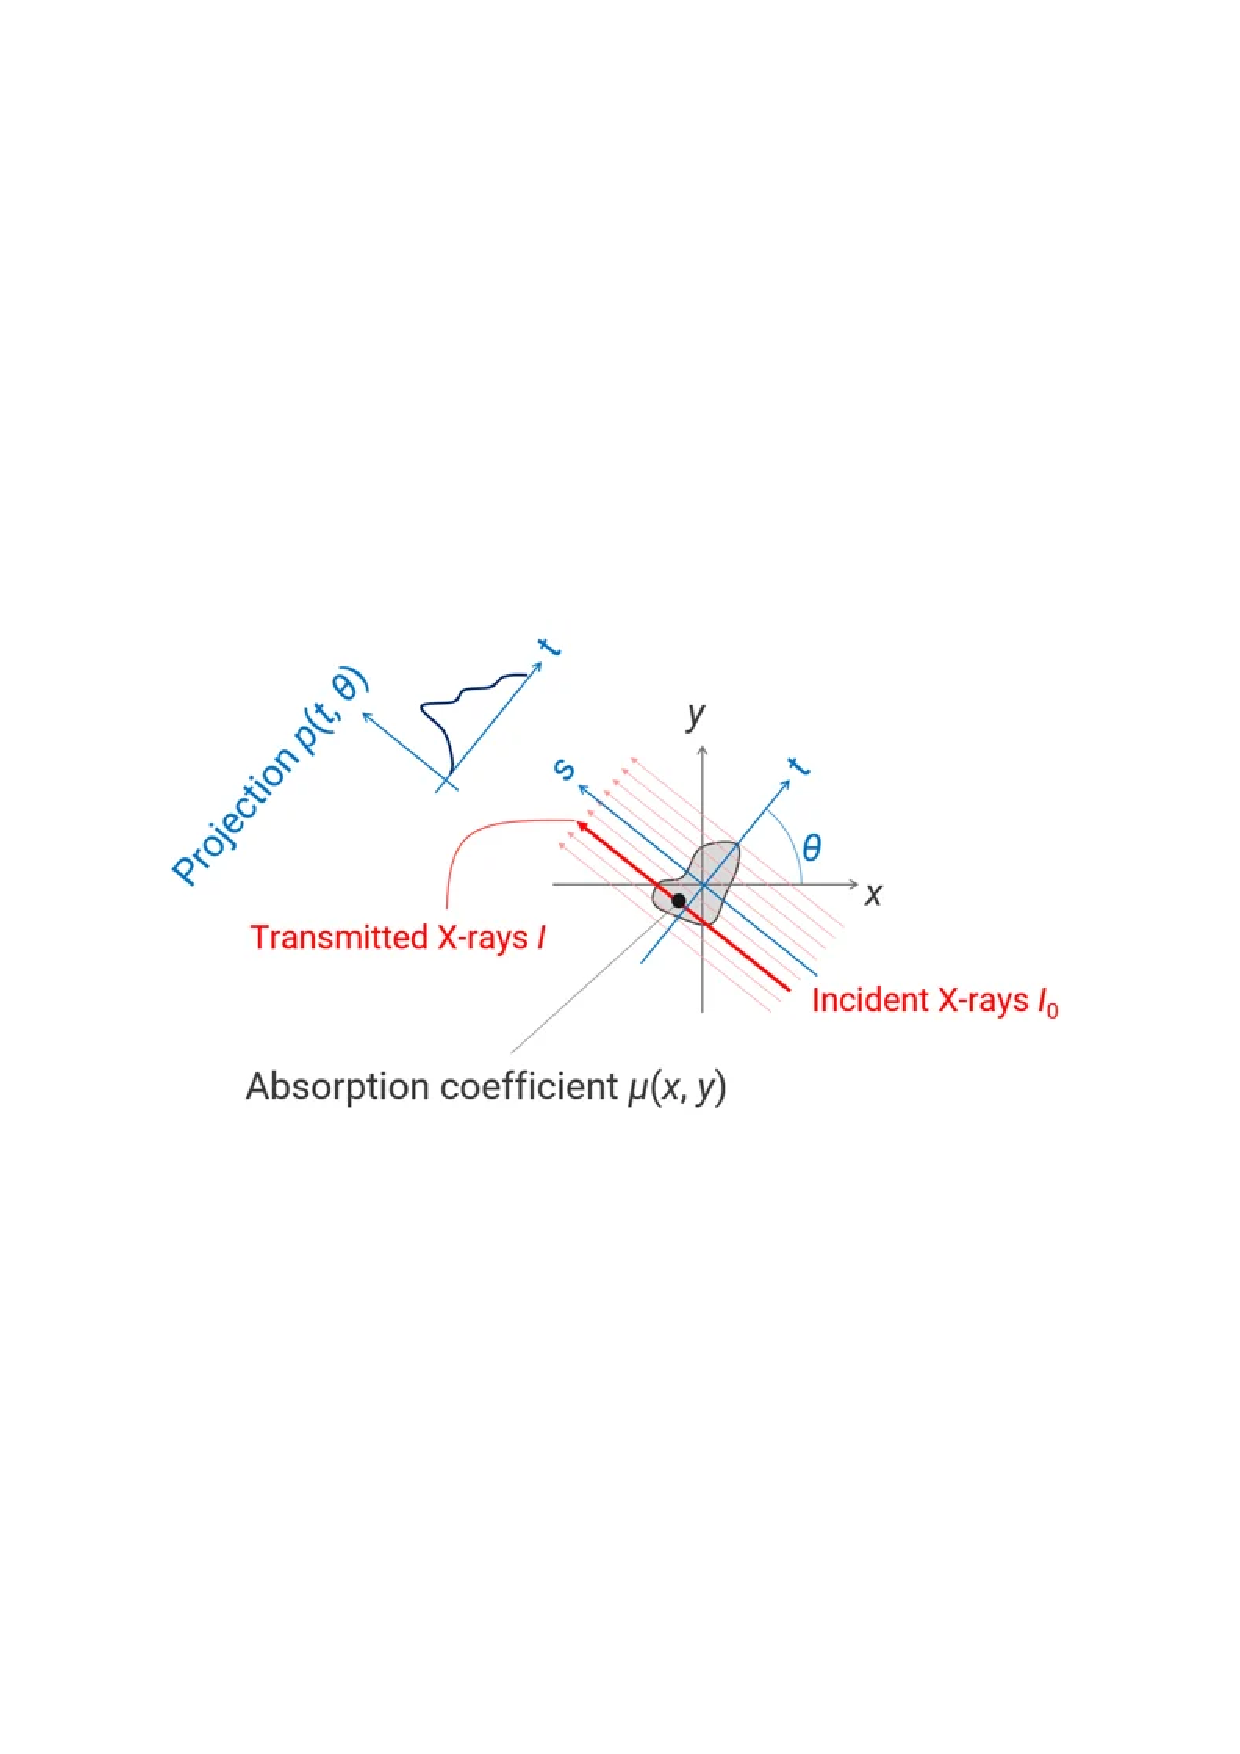
\includegraphics[width=0.5\textwidth,trim={2.5cm 10cm 3cm 10cm}, clip]{img/ct_projection.pdf}
    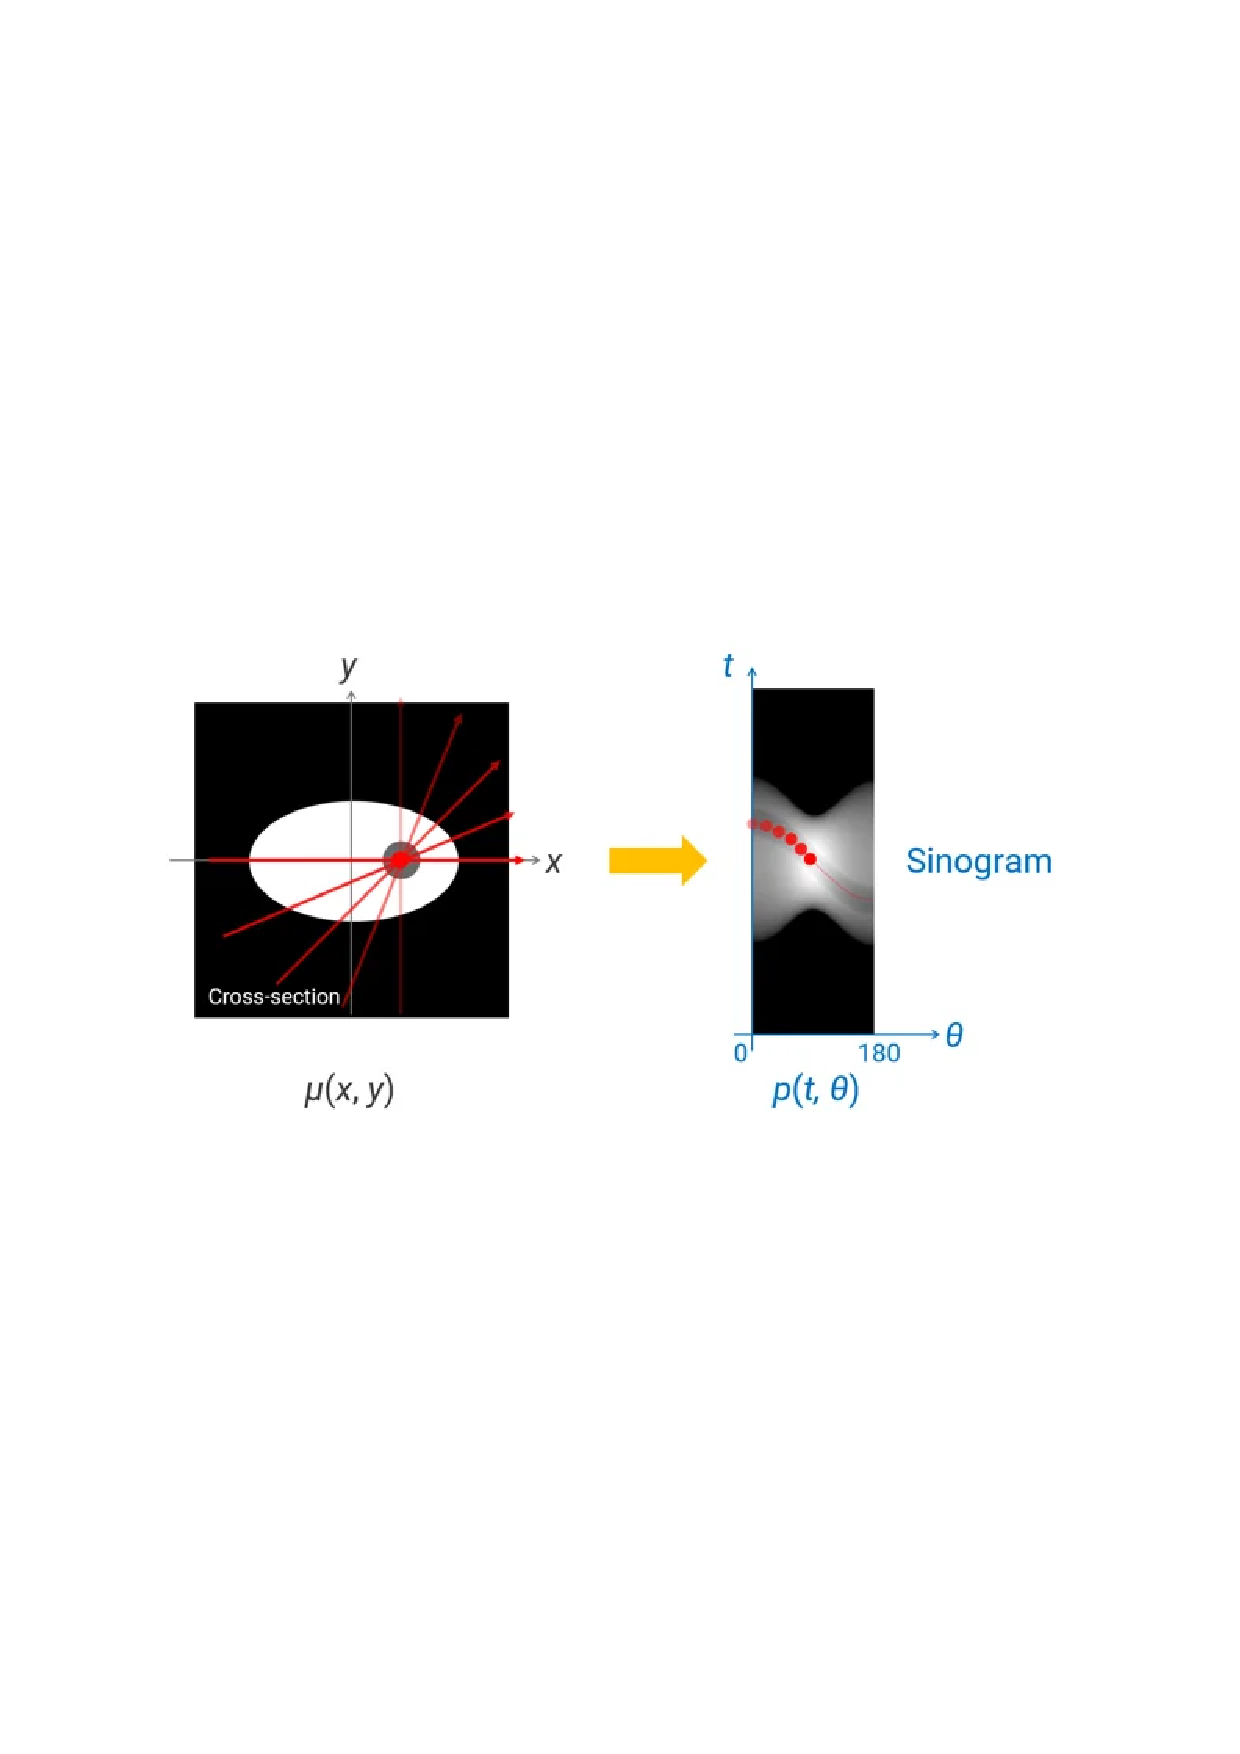
\includegraphics[width=0.4\textwidth,trim={3cm 7cm 3cm 10cm}, clip]{img/ct_sinogram.pdf}
\end{figure}

Kontrast se hodnotí vůči koeficientu zeslabení pro vodu, jednotky Hounsfield. Pokud budu proces opakovat a posouvat spirálou axiálně podél těla $\rightarrow$ dostanu 3D obraz.

\subsubsection{Základní součástky CT tomorgafu}

\begin{itemize}
    \item gantry,
    \item RTG trubice,
    \item kolimátor a filtr,
    \item detektory,
    \item systém získávání informací o odezvě,
    \item vyšetřovací lůžko.
\end{itemize}

\begin{figure}[H]
    \centering
    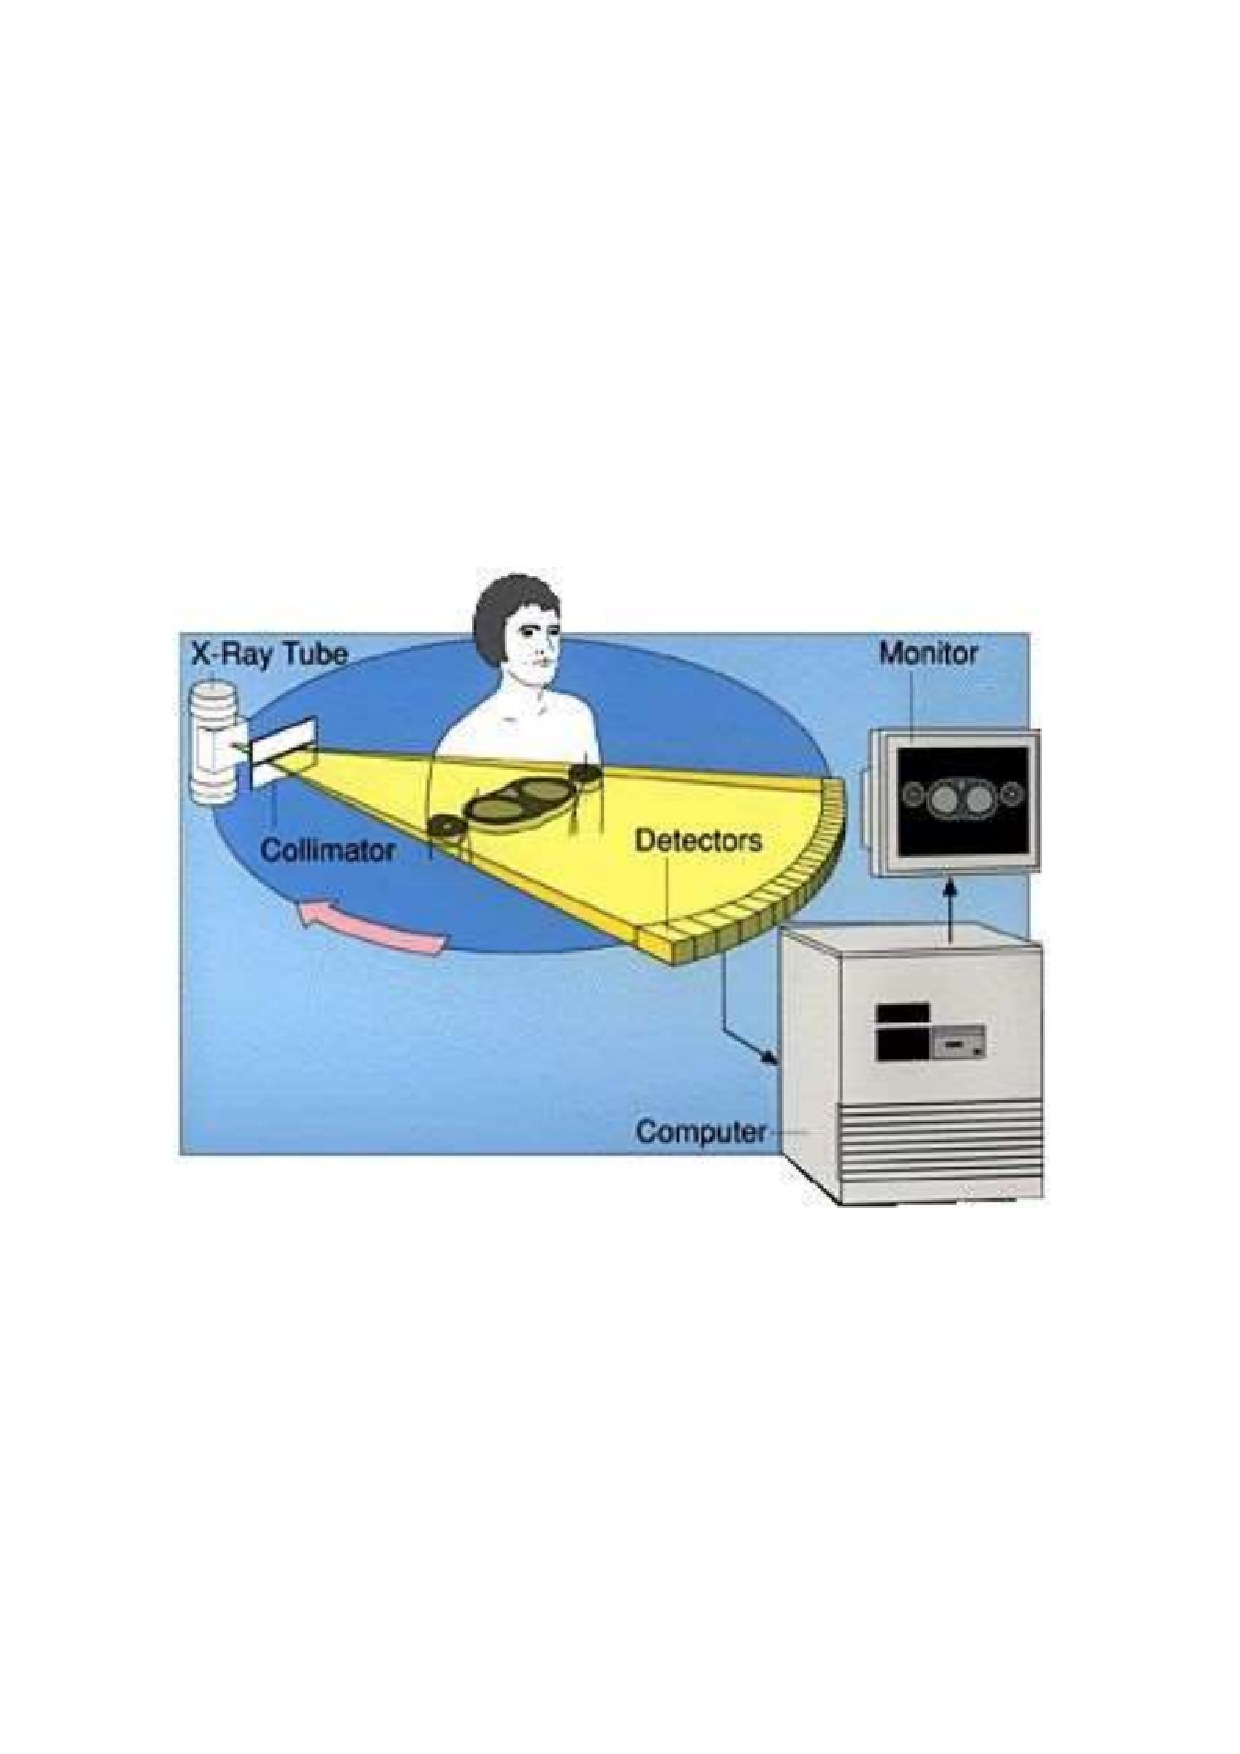
\includegraphics[width=0.5\linewidth,trim={3cm 7cm 3cm 7cm}, clip]{img/ct_ilustrace.pdf}
\end{figure}

\subsection{PET} 

Metoda založená na pozitron-elektronové anihilaci. Zdroj pozitronů $\rightarrow$ beta rozpad.

\subsubsection{Základní součástky PET tomografu}

\begin{itemize}
    \item gantry, 
    \item vyšetřovací lúžko,
    \item systém detektorů, 
    \item počítač,
    \item laserové zaměřovače.
\end{itemize}

Zdroj pozitronů: nejčastěji $^{18}$F v deoxyglukóze. Detektory jsou scintilační detektory (NaI(Tl), berylium germaniový, gadolinium-křemíkový, lutecium-křemíkový), počet detektorů udává rozlišení (tisíce). 

Princip je podobný jako u CT, pomocí detekovaných fotonů z anihilace je pro daný úhel vytvořena projekce, kompletní projekce tvoří sinogram:

$$ \text{sinogram $\rightarrow$ rekonstrukční algoritmus $\rightarrow$ finální obraz.} $$

\subsection{Rozlišení obrazu}

Co narušuje obraz:

\begin{itemize}
    \item útlum -- dáno tloušťkou tkáně, fotoefektem, Comptonovým jevem (sekundární gamma je tlumeno),
    \item Comptonův rozptyl,
    \item náhodná koincidence.
\end{itemize}

Často mohu kombinovat CT a PET. Z CT získám anatomickou strukturu, z PET biologické procesy.


\begin{figure}[H]
    \centering
    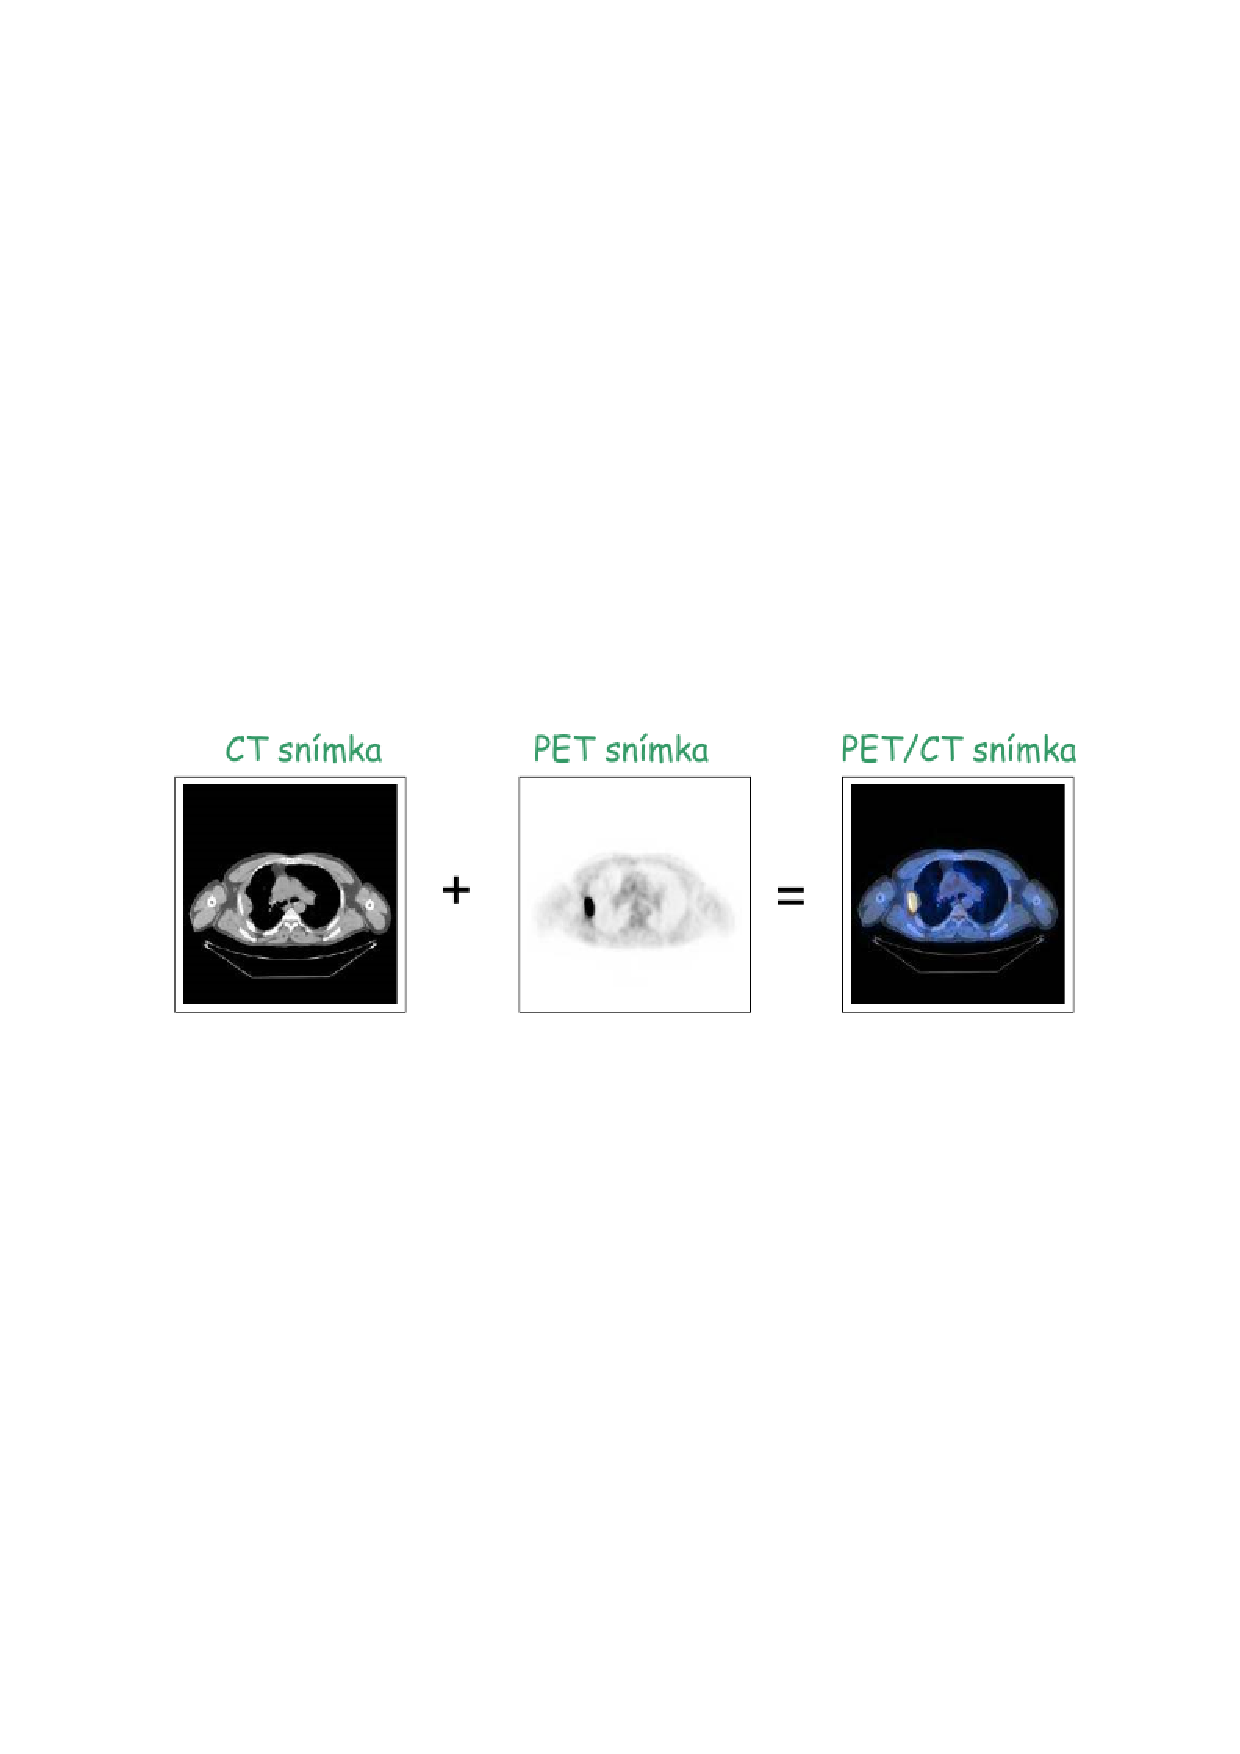
\includegraphics[width=0.8\linewidth, trim={1cm 11cm 1cm 11cm}, clip]{img/pet_obrazy.pdf}
    \caption{Snímky z CT a PET tomografie}
    \label{fig:2_6_CT_PET_tomografie}
\end{figure}